\chapter{Collectivity in QCD}
\section{Conceptual Understanding of Collectivity and Flow}
The observation of collectivity in matter can be a powerful indicator of fundamental properties in that matter. Collectivity means many discrete structures are interacting together to form a whole. In high energy heavy ion physics, collectivity can be thought of as a medium formed that can be described as a locally equilibrated system evolving hydrodynamically instead of a group of individually interacting constituents. Collectivity is measured by looking for long-range angular correlations in the spray of final state particles that come out of the collision. A key property of high energy heavy ion collisions is that information on the initial conditions will be carried through the medium evolution. Thus, an asymmetry in the initial conditions of the heavy ion collision is measurable in the final products
\begin{figure}[h!]
\begin{center}
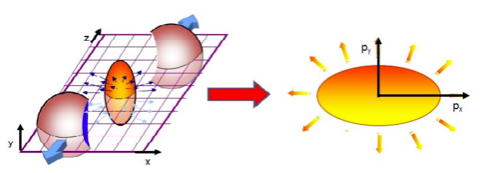
\includegraphics[width=0.45\linewidth]{figs/elliptical_flow_cartoon.png}
\caption{ TBA }
\end{center}
\end{figure}

\section{Mathematical Introduction}
A measurement of the azimuthal anisotropy is a way to quantify the extent of long-range angular correlation present in the medium evolution. Features of azimuthal anisotropy can be studied by creating a correlation function. The 2-particle correlation function method uses pairs of particles from the event in order to create a correlation function. For each each pair in an event, a $\Delta\phi$ value is obtained which makes up the signal $S(\Delta\phi,p_T)$. In order to correct for artificial correlations which would distort the distribution from detector effects or other sources, a mixed event background distribution $M(\Delta\phi,pT)$ is created. The correlation function can be defined as follows:

%\begin{equation}\label{eqn:corr_func}
%  C(\Delta,p_T) = \frac{S(\Delta\phi,p_T)}{M(\Delta\phi,p_T)}\frac{\int_{0}^{2\pi}M(\Delta\phi,p_T)d\Delta\phi)}{\int_0^{2\pi}S(\Delta\phi,p_T)d\Delta\phi)}
%\end{equation}

%multi particle cumulants - later
%correlation function
%describe c2 vs v2

\begin{eqnarray}
  S(\Delta\phi,p_{T})=
  \frac{ d(w_{{\rm PMT}} N^{{\rm track}(p_{T}){\rm - PMT}}_{{\rm Same \; event}}) }{ d\Delta\phi}, & &
\label{eq31} \\
  C(\Delta\phi,p_{T}) =
          \frac{S(\Delta\phi,p_{T})}{M(\Delta\phi,p_{T})} \:
          \frac{\int_{0}^{2\pi} M(\Delta\phi,p_{T}) \, d\Delta\phi}{\int_{0}^{2\pi} S(\Delta\phi,p_{T}) \, d\Delta\phi}. & &
  \label{eq:def_corr_function}
\end{eqnarray}

Substantial variations in this $C(\Delta\phi,p_T)$ are usually seen as long-range angular correlations which can be attributed to collectivity.

In order to quantify the azimuthal anisotropy, $C(\Delta\phi,p_T)$ is Fourier transformed:
\begin{equation}\label{eqn:dndphi}
  C(\Delta\phi,p_T) \propto 1 + \sum_{n=1}2 v_{n}\cos(n[\phi(p_T)-\Psi_n]) 
\end{equation}

where $\Psi_n$ is the event plane angle, $\phi$ is the azimuth of tracks from the event, and $v_n$ are flow coefficients. The measured $v_n$ averaged over a single event is defined as:
\begin{equation}\label{eqn:vn}
  v_n = \frac{\langle\cos(n[\phi-\Psi_n])\rangle}{Res(\Psi_n)}
\end{equation}

where $Res(\Psi_n)$ is the event plane resolution for each event. $v_N$ are further averaged over each event.
\begin{equation}
\varepsilon_n = \frac{\sqrt{\langle r^2\cos (n\phi)\rangle ^2 + \langle r^2\sin (n\phi) \rangle ^2}}{\langle r^2 \rangle}
\end{equation}

\begin{figure}[h!]
\begin{center}
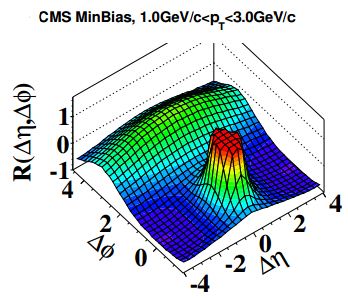
\includegraphics[width=0.45\linewidth]{figs/pp_correlation_function_min_bias.png}
\caption{ }
\label{fig:pp_corr_func_minbias}
\end{center}
\end{figure}

The significance of a the so called ``near-side ridge" is due to the fact that region in $\Delta\phi$, $\Delta\eta$ space can only be comprised of pairs of particles with long range angular correlations unassociated with any known non-flow effects.

\section{A Review of Flow Measurements in Small Collision Systems}
%p+p ridge
%he3au v3
%pPb
%other experiments
% mass ordering

As mentioned at the end of Chapter 1, small collision systems have been considered too small to create hot and dense matter. These systems were used as control experiments which could be used to measure how the presence of a nucleus would effect the production of particles relative to $p+p$ collisions. These so called "cold nuclear matter" (CNM) effects would be isolated when colliding very low $Z$ nuclei, such as a deuteron or proton, with a large nucleus.\footnote{ A quick side note: the convention in the field of heavy ion physics is to label any such small system collisions as $p$+A and any large system collisions as A+A} Generally accepted CNM effects are: nuclear shadowing which is the modification of parton distribution functions by a nucleus, gluon saturation, radiative energy loss which is the modification of the momentum fraction of partons due to multiple soft scatterings, and finally the Cronin effect which is the broadening of the transverse momentum of emitted particles distribution due to multiple scatterings of initially colliding partons \textbf{add ref}.  

In 2010, the CMS collaboration published a paper observing a nearside ridge in high multiplicity 7 TeV $p+p$ events in the correlation function for dihadrons as shown in Figure \ref{fig:pp_ridge_plot}. The aforementioned nearside ridge is located at $\Delta\phi$ = 0 and at $|\Delta\eta| > $ 2 in the figure. The ridge is significant in contrast to the minimum bias $p+p$ correlation function shown in Figure \ref{fig:pp_corr_func_minbias} with an absence of any such ridge.
\begin{figure}[h!]
\begin{center}
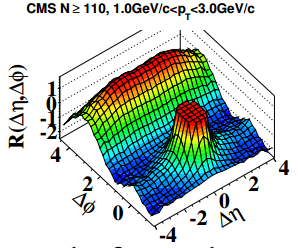
\includegraphics[width=0.55\linewidth]{figs/pp_high_multiplicity_ridge.PNG}
\caption{ The correlation function for $p+p$ collisions at \sqsn = 7 TeV for hadrons with 1.0 $<|p_T|<$ 3.0 GeV/c in high multiplicity events with greater than 109 charged particle tracks were found \cite{Khachatryan2010}.}
\label{fig:pp_ridge_plot}
\end{center}
\end{figure}

\begin{figure}[h!]
\begin{center}
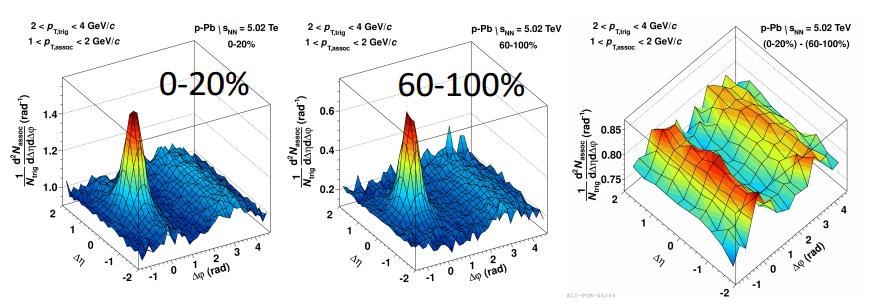
\includegraphics[width=0.85\linewidth]{figs/pPb_subtraction_correlation.PNG}
\caption{ The correlation function for $p+p$ collisions at \sqsn = 7 TeV for hadrons with 1.0 $<|p_T|<$ 3.0 GeV/c in high multiplicity events with greater than 109 charged particle tracks were found \cite{Khachatryan2010}.}
\label{fig:pp_ridge_plot}
\end{center}
\end{figure}

\begin{figure}[h!]
\begin{center}
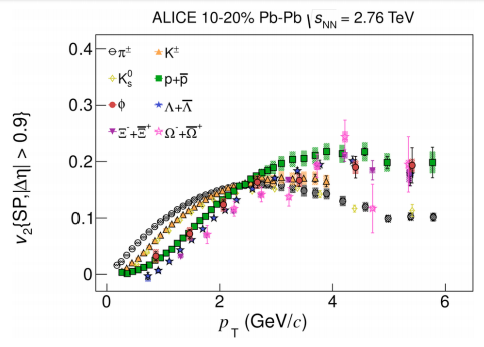
\includegraphics[width=0.48\linewidth]{figs/PbPb_v2_mass_ordering.PNG}
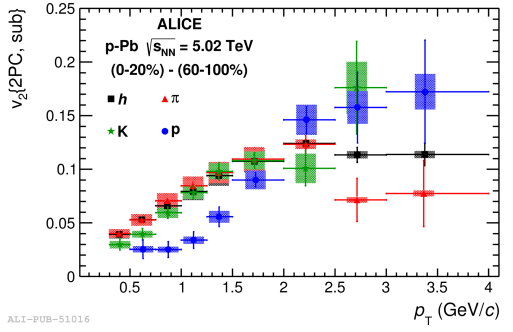
\includegraphics[width=0.48\linewidth]{figs/pPb_two_part_v2_mass_ordering.PNG}
\caption{ The correlation function for $p+p$ collisions at \sqsn = 7 TeV for hadrons with 1.0 $<|p_T|<$ 3.0 GeV/c in high multiplicity events with greater than 109 charged particle tracks were found \cite{Khachatryan2010}.}
\label{fig:pp_ridge_plot}
\end{center}
\end{figure}

\begin{figure}[h!]
\begin{center}
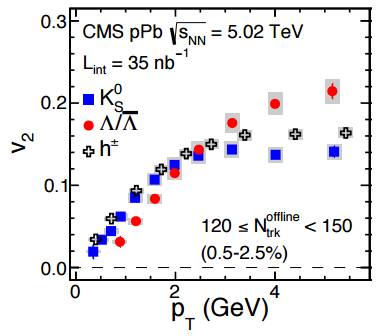
\includegraphics[width=0.55\linewidth]{figs/pBp_v2_mass_ordering.PNG}
\caption{ CMS The correlation function for $p+p$ collisions at \sqsn = 7 TeV for hadrons with 1.0 $<|p_T|<$ 3.0 GeV/c in high multiplicity events with greater than 109 charged particle tracks were found \cite{Khachatryan2010}.}
\label{fig:pp_ridge_plot}
\end{center}
\end{figure}

\begin{figure}[h!]
\begin{center}
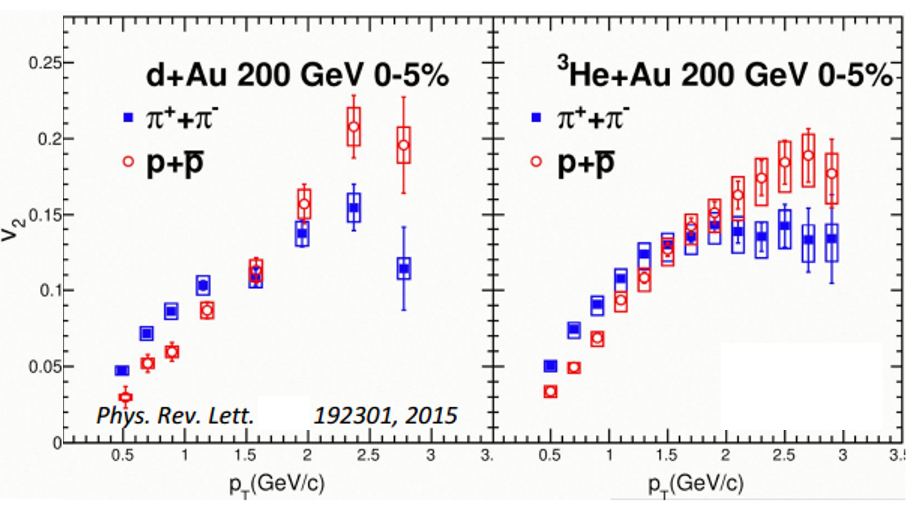
\includegraphics[width=0.65\linewidth]{figs/dhau_mass_ordering_phenix.PNG}
\caption{ The correlation function for $p+p$ collisions at \sqsn = 7 TeV for hadrons with 1.0 $<|p_T|<$ 3.0 GeV/c in high multiplicity events with greater than 109 charged particle tracks were found \cite{Khachatryan2010}.}
\label{fig:pp_ridge_plot}
\end{center}
\end{figure}

\begin{figure}[h!]
\begin{center}
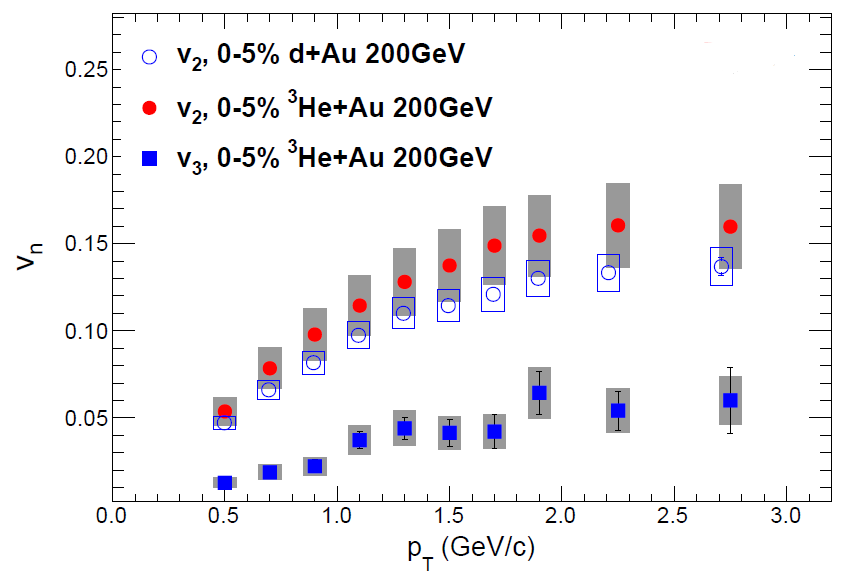
\includegraphics[width=0.75\linewidth]{figs/hedau_v2_v3.PNG}
\caption{ The correlation function for $p+p$ collisions at \sqsn = 7 TeV for hadrons with 1.0 $<|p_T|<$ 3.0 GeV/c in high multiplicity events with greater than 109 charged particle tracks were found \cite{Khachatryan2010}.}
\label{fig:pp_ridge_plot}
\end{center}
\end{figure}

\begin{figure}[h!]
\begin{center}
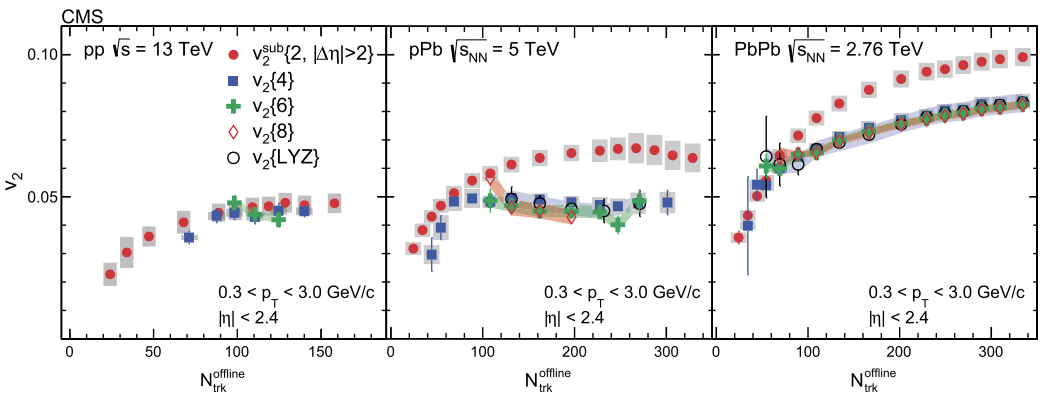
\includegraphics[width=0.65\linewidth]{figs/pp_pPb_PbPb_cumulants.PNG}
\caption{ The correlation function for $p+p$ collisions at \sqsn = 7 TeV for hadrons with 1.0 $<|p_T|<$ 3.0 GeV/c in high multiplicity events with greater than 109 charged particle tracks were found \cite{Khachatryan2010}.}
\label{fig:pp_ridge_plot}
\end{center}
\end{figure}

However, evidence of collectivity has recently been observed at RHIC in p+Au collisions at $\sqrt{s_{NN}}$ = 200 GeV in the most central collisions ~\cite{PhysRevLett.115.142301}. Although, the $p_T$ dependent $v_N$ has been measured, what has not been measured in these small systems is the degree to which $v_N$ changes a function of rapidity. This is a particularly interesting measurement to make in an asymmetric collision system such as p+Au.

Recent analyses of d+Au and HeAu collisions at $\sqrt{n}$ = 200 GeV~\cite{PhysRevLett.111.212301,Adare:2014keg,Adare:2015ctn,Adamczyk:2014fcx} at the Relativistic Heavy-Ion Collider (RHIC), and p+Pb at $\sqrt{n}$ = 5.02 TeV, and $p+p$ collisions at $\sqrt{n}$ = 2.76, 5.02, 7, and 13 TeV~\cite{alice_long_2013,atlas_observation_2012,cms_observation_2012,Khachatryan:2015lva,Aad:2015gqa,Khachatryan:2010gv,Khachatryan:2016txc} at the Large Hadron Collider (LHC) have demonstrated the existence of the same kind of azimuthal anisotropy signals commonly interpreted as evidence of collective behavior in larger systems. Notably, a feature known as \textit{the ridge} has been observed, consisting of a near-side (i.e., at small relative azimuth) enhancement in the long-range (i.e., at large relative pseudorapidity) azimuthal two-particle correlation. From these correlations, substantial elliptic ($v_2$), and triangular ($v_3$) flow coefficients have been measured in these systems.

\section{An Overview of Simulations}

\subsection{Initial Condition}
\subsubsection{Monte-Carlo Initial Condition Characterization}
\begin{figure}[h!]
\begin{center}
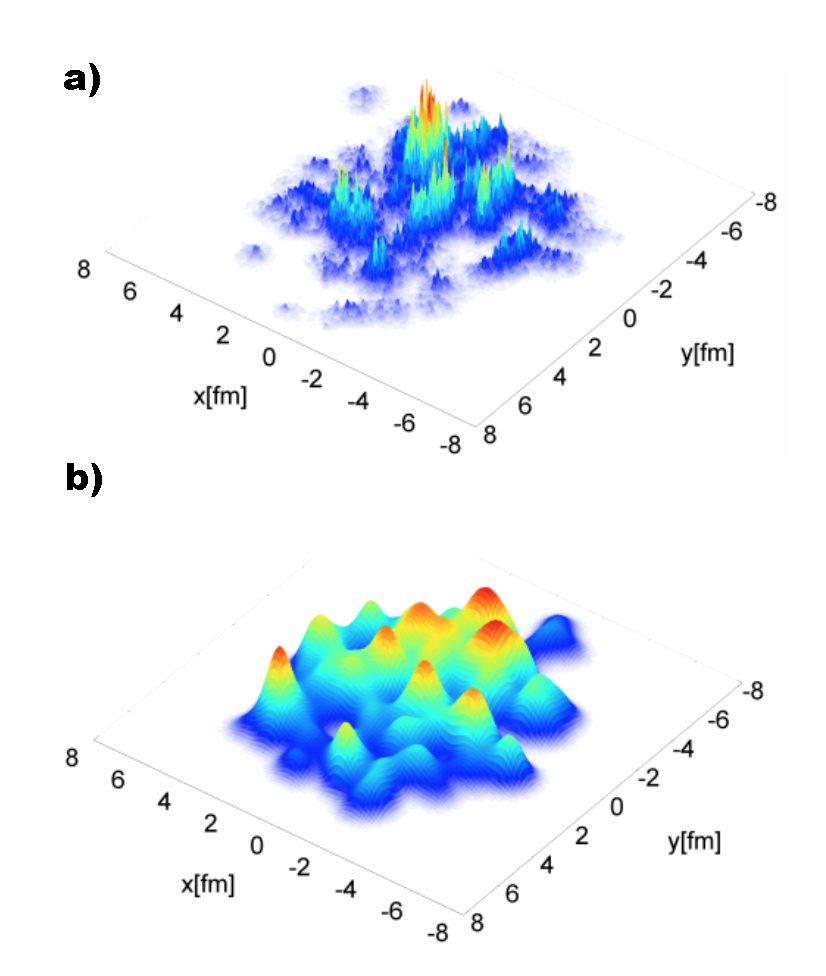
\includegraphics[width=0.45\linewidth]{figs/initial_conditions.png}
\caption{ a) IP-glasma. b) MC-KLN. c) MC-Glauber.}
\end{center}
\end{figure}

\begin{figure}[h!]
\begin{center}
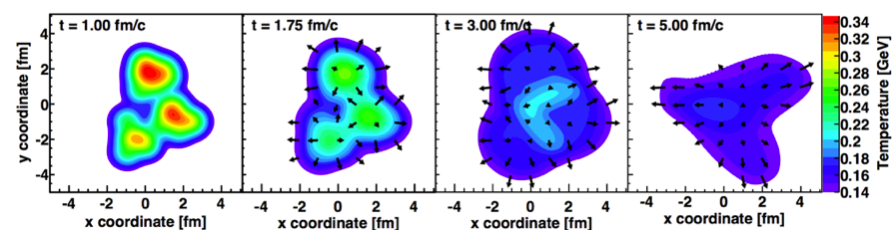
\includegraphics[width=0.45\linewidth]{figs/he3au_simulation.png}
\caption{ TBA }
\end{center}
\end{figure}

\subsubsection{IP Glasma}

\subsection{Hydrodynamic Treatment}

\subsubsection{SONIC}

\subsubsection{SuperSONIC}

\subsection{AMPT}